\documentclass[zihao=-4]{ctexart}
\usepackage[normalem]{ulem}
\useunder{\uline}{\ul}{}
%********************导言区宏包引入********************
\usepackage{xeCJK}
\usepackage{amssymb}
\usepackage{amsmath}
\usepackage{listings} %代码
\usepackage{graphicx}
\usepackage{multicol} %回车换段
\usepackage{xcolor}
\usepackage{geometry} %页面设置
\usepackage{fontspec}
\usepackage{setspace}
\usepackage{times}
\usepackage{fancyhdr} %页眉页脚
\pagestyle{fancy}
\usepackage{float} %表格位置
\usepackage{titlesec} %设置
\usepackage{titletoc}
\usepackage{ctex}
\usepackage{gbt7714}    %控制参考文献格式为国标
\usepackage{multirow}
\usepackage{booktabs}   %表格相关
\usepackage{setspace}   %设置行距
\usepackage{caption} %caption
\usepackage{subcaption} %子图的caption
\usepackage{changepage} %左右缩进

% for 代码
\definecolor{mygreen}{rgb}{0,0.6,0}
\definecolor{mygray}{rgb}{0.5,0.5,0.5}
\definecolor{mymauve}{rgb}{0.58,0,0.82}


\graphicspath{ {include_picture/} }
\let\algorithm\relax
\let\endalgorithm\relax
\usepackage[ruled,vlined]{algorithm2e}%[ruled,vlined]{
\usepackage{algpseudocode}
\renewcommand{\algorithmicrequire}{\textbf{Input:}} 
\renewcommand{\algorithmicensure}{\textbf{Output:}}
%\renewcommand\thepage{\zihao{-5} ~\arabic{page}~}%页码字号

%定义两个arg
\DeclareMathOperator*{\argmax}{arg\,max}
\DeclareMathOperator*{\argmin}{arg\,min}
\DeclareCaptionLabelSeparator{mysep}{\space\space}  %自定义caption格式
\captionsetup[figure]{font={small}, labelfont=bf, labelsep=mysep, textfont=bf}   %图片caption格式
\captionsetup[table]{font={small}, labelfont=bf, labelsep=mysep, textfont={bf}}   %表格caption格式
\bibliographystyle{gbt7714-numerical} %修改了title斜体内容

%********************导言区宏包引入********************
% Use TeX Live fonts; original proprietary font files are not redistributed.
\setmainfont{TeX Gyre Termes}
\setmonofont{TeX Gyre Cursor}
\setCJKfamilyfont{hwzs}{FandolSong-Regular}
\newcommand{\zhongsong}{\CJKfamily{hwzs}}
\setCJKfamilyfont{hwxw}{FandolKai-Regular}
\newcommand{\xinwei}{\CJKfamily{hwxw}}

%********************中文字号设置********************
%\newcommand{\chuhao}{\fontsize{42pt}{\baselineskip}\selectfont}
\newcommand{\chuhao}{\fontsize{42pt}{0}}
\newcommand{\xiaochu}{\fontsize{36pt}{0}}
\newcommand{\yihao}{\fontsize{28pt}{0}}
\newcommand{\erhao}{\fontsize{21pt}{0}}
\newcommand{\xiaoer}{\fontsize{18pt}{0}}
\newcommand{\sanhao}{\fontsize{16pt}{0}}
\newcommand{\sihao}{\fontsize{14pt}{0}}
\newcommand{\xiaosi}{\fontsize{12pt}{0}}
\newcommand{\wuhao}{\fontsize{10.5pt}{0}}
\newcommand{\xiaowu}{\fontsize{9pt}{0}}
\newcommand{\liuhao}{\fontsize{8pt}{0}}
\newcommand{\qihao}{\fontsize{5.25pt}{0}}

% 个人信息 自定义命令 固定长度下划线
\newcommand\ful[2][4cm]{\underline{\makebox[#1][c]{#2}}}
%********************中文字号设置********************


%********************代码段********************
% https://www.cnblogs.com/PiaYie/p/15720770.html
\lstset{ %
  backgroundcolor=\color{white},   % choose the background color; you must add \usepackage{color} or \usepackage{xcolor}
  basicstyle=\footnotesize,        % the size of the fonts that are used for the code
  breakatwhitespace=false,         % sets if automatic breaks should only happen at whitespace
  breaklines=true,                 % sets automatic line breaking
  captionpos=bl,                    % sets the caption-position to bottom
  commentstyle=\color{mygreen},    % comment style
  deletekeywords={...},            % if you want to delete keywords from the given language
  escapeinside={\%*}{*)},          % if you want to add LaTeX within your code
  extendedchars=true,              % lets you use non-ASCII characters; for 8-bits encodings only, does not work with UTF-8
  frame=single,                    % adds a frame around the code
  keepspaces=true,                 % keeps spaces in text, useful for keeping indentation of code (possibly needs columns=flexible)
  keywordstyle=\color{blue},       % keyword style
  %language=Python,                 % the language of the code
  morekeywords={*,...},            % if you want to add more keywords to the set
  numbers=left,                    % where to put the line-numbers; possible values are (none, left, right)
  numbersep=5pt,                   % how far the line-numbers are from the code
  numberstyle=\tiny\color{mygray}, % the style that is used for the line-numbers
  rulecolor=\color{black},         % if not set, the frame-color may be changed on line-breaks within not-black text (e.g. comments (green here))
  showspaces=false,                % show spaces everywhere adding particular underscores; it overrides 'showstringspaces'
  showstringspaces=false,          % underline spaces within strings only
  showtabs=false,                  % show tabs within strings adding particular underscores
  stepnumber=1,                    % the step between two line-numbers. If it's 1, each line will be numbered
  stringstyle=\color{orange},     % string literal style
  tabsize=2,                       % sets default tabsize to 2 spaces
  literate={-}{{\textendash}}{1}
  %title="No name code"                   % show the filename of files included with \lstinputlisting; also try caption instead of title
}
%********************代码段********************


%********************页边距设置********************
\geometry{left=3cm,right=2cm,top=2.5cm,bottom=2.5cm}
\geometry{a4paper} % xsp 2023/3/7: 调整纸张大小为A4
%********************页边距设置********************

%********************段间距设置********************
\newcommand{\setParDis}{\setlength {\parskip} {0pt} }
%请在每部分使用这个
%********************段间距设置********************

%********************

\begin{document}
%********************页眉页脚设置********************
\lhead{}%设置左页眉为空
\rhead{}%设置左页眉为空
\setlength{\headwidth}{\textwidth}% 2023/3/3 XSP: 页眉长度适应文本
%********************页眉页脚设置********************


%********************标题格式设置********************

%\setcounter{secnumdepth}{0}%该命令取消了章标题前数字label

\CTEXsetup[name={,、},number={\chinese{section}}]{section}
\CTEXsetup[name={（,）},number={\chinese{subsection}}]{subsection}
\CTEXsetup[name={,.},number={\arabic{subsubsection}}]{subsubsection}% 不加会导致目录格式错误
% 设置subsubsection等格式
% \titleformat{\section}[block]{\sanhao\bfseries\centering}{\chinese{section}、}{0pt}{}[]
% \titleformat{\subsection}[block]{\sihao\bfseries}{（\chinese{subsection}）}{0pt}{}[]
% \titleformat{\subsubsection}[block]{\xiaosi\bfseries}{\arabic{subsubsection}、}{0pt}{}[]
\titleformat{\section}[block]{\sanhao\heiti\centering}{\chinese{section}、}{0pt}{}[]    % XSP 2023/3/3:
\titleformat{\subsection}[block]{\sihao\heiti}{（\chinese{subsection}）}{0pt}{}[]       %   将正文标题字体由加粗
\titleformat{\subsubsection}[block]{\xiaosi\heiti}{\arabic{subsubsection}.}{0pt}{}[]   % 修改为黑体。
\titlespacing{\section}{0pt}{25pt}{12pt}
\titlespacing{\subsection}{0pt}{7pt}{7pt}
\titlespacing{\subsubsection}{0pt}{5pt}{4pt}

\titlecontents{section}[1.6em]{\addvspace{2pt}\filright}
{\contentspush{\thecontentslabel\hspace{0.8em}}}
{}{\titlerule*[8pt]{.}\contentspage}

\titlecontents{subsection}[3.2em]{\addvspace{2pt}\filright}
{\contentspush{\thecontentslabel\hspace{0.8em}}}
{}{\titlerule*[8pt]{.}\contentspage}

\titlecontents{subsubsection}[6.4em]{\addvspace{2pt}\filright}
{\contentspush{\thecontentslabel\hspace{0.8em}}}
{}{\titlerule*[8pt]{.}\contentspage}
%********************标题格式设置********************

%\setcounter{section}{-3}  %标题计数器
%\stepcounter{section}

%*******************行间距段前段后*******************
\linespread{1.8}
%行间距为实际行间距乘以1.2,如此处实际为1.5倍行距
\setlength{\parskip}{0.5\baselineskip}
%*******************行间距段前段后*******************



% Identifying course cover removed during archival cleanup.
\renewcommand{\headrulewidth}{0pt}
\pagenumbering{roman} %摘要目录页小写罗马

\xiaosi




%********************摘要部分********************


%********************目录部分********************
\clearpage
\tableofcontents
\clearpage
%********************目录部分********************



\renewcommand{\headrulewidth}{0.4pt} %恢复页眉装饰线

%********************正文页眉部分********************
%\lhead{} 
\chead{\xiaowu \CourseName 实验报告} %设置居中页眉
%********************正文页眉部分********************

\pagenumbering{arabic} %正文页码从1开始，用阿拉伯数字
\setcounter{page}{1} 

\section{串行代码解读}
\setParDis %设置段间距为 0
\begin{spacing}{1.5}

\subsection{数据结构}

该程序中声明了数种结构体，定义了结构体类型的多个变量，以存储文法的相关信息和CYK算法的数据。

\subsubsection{二元产生式}

二元产生式结构体Production2，其声明代码如下。

\begin{lstlisting}[language=C++,title={二元产生式声明与定义}]
struct Production2 {
    int parent;
    int child1;
    int child2;
} production2[MAX_PRODUCTION2_NUM];
\end{lstlisting}

这段代码也同时定义了该结构体类型的数组变量production2，用于存储Chomsky范式中的二元产生式。其中parent表示产生式的父节点（非终结符），child1表示产生式的第一个子节点（非终结符），child2表示产生式的第二个子节点（非终结符）。

\subsubsection{一元产生式}

一元产生式结构体Production2，其声明代码如下。

\begin{lstlisting}[language=C++,title={一元产生式声明与定义}]
struct Production1 {
    int parent;
    char child;
} production1[MAX_PRODUCTION1_NUM];
\end{lstlisting}

这段代码也同时定义了该结构体类型的数组变量production1，用于存储Chomsky范式中的一元产生式。parent表示产生式的父节点（非终结符），child表示产生式的子节点（终结符）。

\subsubsection{产生式索引}

算法在搜索产生式时，使用的是产生式右侧的符号组合，查找是否有产生式能够生成待搜索的右侧符号，或者说待搜索的右侧符号组合是否能够规约成为一个非终结符。为了加速产生式的搜索过程，程序依照右侧符号也就是搜索键，为输入的产生式进行排序，同时使用产生式索引。以下代码声明了产生式索引的结构体。

\begin{lstlisting}[language=C++,title={产生式索引结构体声明}]
struct BeginAndNum
{
    int begin;
    unsigned num;
};
\end{lstlisting}

该结构体用于存储开始索引和数量。begin表示目标产生式的开始索引，num表示数量。定义了两个该类型的数组变量，用于存放产生式索引。

\begin{lstlisting}[language=C++,title={产生式索引变量定义}]
BeginAndNum vnIndex[MAX_VN_NUM][MAX_VN_NUM];
BeginAndNum vtIndex[MAX_VT_NUM];
\end{lstlisting}

vnIndex用于存储二元产生式的索引信息，指出其在production2数组中的位置，当需要查找child1和child2能生成哪些非终结符时，可以直接通过vnIndex快速定位到这些产生式，而不需要遍历整个产生式数组。vtIndex用于存储一元产生式的索引信息，指出其在production1数组中的位置，当需要查找某个终结符t能生成哪些非终结符时，可以直接通过vtIndex快速定位到这些产生式。

\subsubsection{语法子树}

程序声明以下结构体，用以存储子树根节点的非终结符，以及该子树可能的结构数量。需要注意的是，我们不保存完整的子树结构，仅仅记录数量。

\begin{lstlisting}[language=C++,title={子树声明与定义}]
struct SubTree
{
    int root;
    unsigned num;
} subTreeTable[MAX_STRING_LENGTH][MAX_STRING_LENGTH][MAX_VN_NUM];
\end{lstlisting}

其中root表示子树的根节点（非终结符），num表示子树的数量。同时定义的subTreeTable数组中保存了输入字符串的子串的对应语法子树，具体来说subTreeTable[i][j]表示下标范围[i, j]（从0开始）的子串能够规约形成的非终结符及对应子树的数量。

\subsection{算法理解}

\subsubsection{算法核心过程}

下图即为CYK算法伪代码。

\begin{figure}[H] %H为当前位置，!htb为忽略美学标准，htbp为浮动图形
    \centering %图片居中
    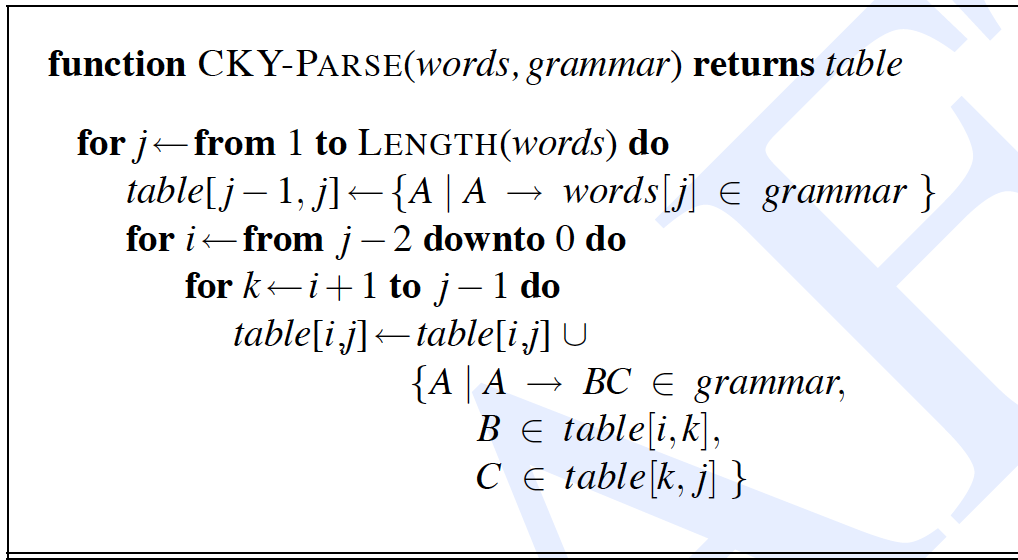
\includegraphics[width=0.8\textwidth]{include_picture/code.png} %插入图片，[]中设置图片大小，{}中是图片文件名
    \caption{CYK算法伪代码} %最终文档中希望显示的图片标题
    \label{fake_code} %用于文内引用的标签
\end{figure}

对于这份伪代码，table[i, j]中保存的即为下标范围[i, j)（从0开始）的子串所能规约到的非终结符。

在外层循环中，j从1到LENGTH(words)，初始化每个单字符子串的位置。对于每个字符 words[j]，如果存在产生式A:=words[j]，则将A放入table[j-1, j]中，表明第j（从1开始）个字符，能够被规约成哪些非终结符。在中层循环中，i从j-2递减到0，表明对于每一列，我们从下向上进行处理。在内层循环中，对于每个可能的起始位置i，遍历所有可能的划分点k，检查是否存在产生式A:=BC，其中B是table[i, k]中的一个非终结符，C是table[k, j]中的一个非终结符。如果存在，则将A添加到table[i, j]中。下图是示例的文法、输入串和算法执行结果。

\begin{figure}[H] %H为当前位置，!htb为忽略美学标准，htbp为浮动图形
    \centering %图片居中
    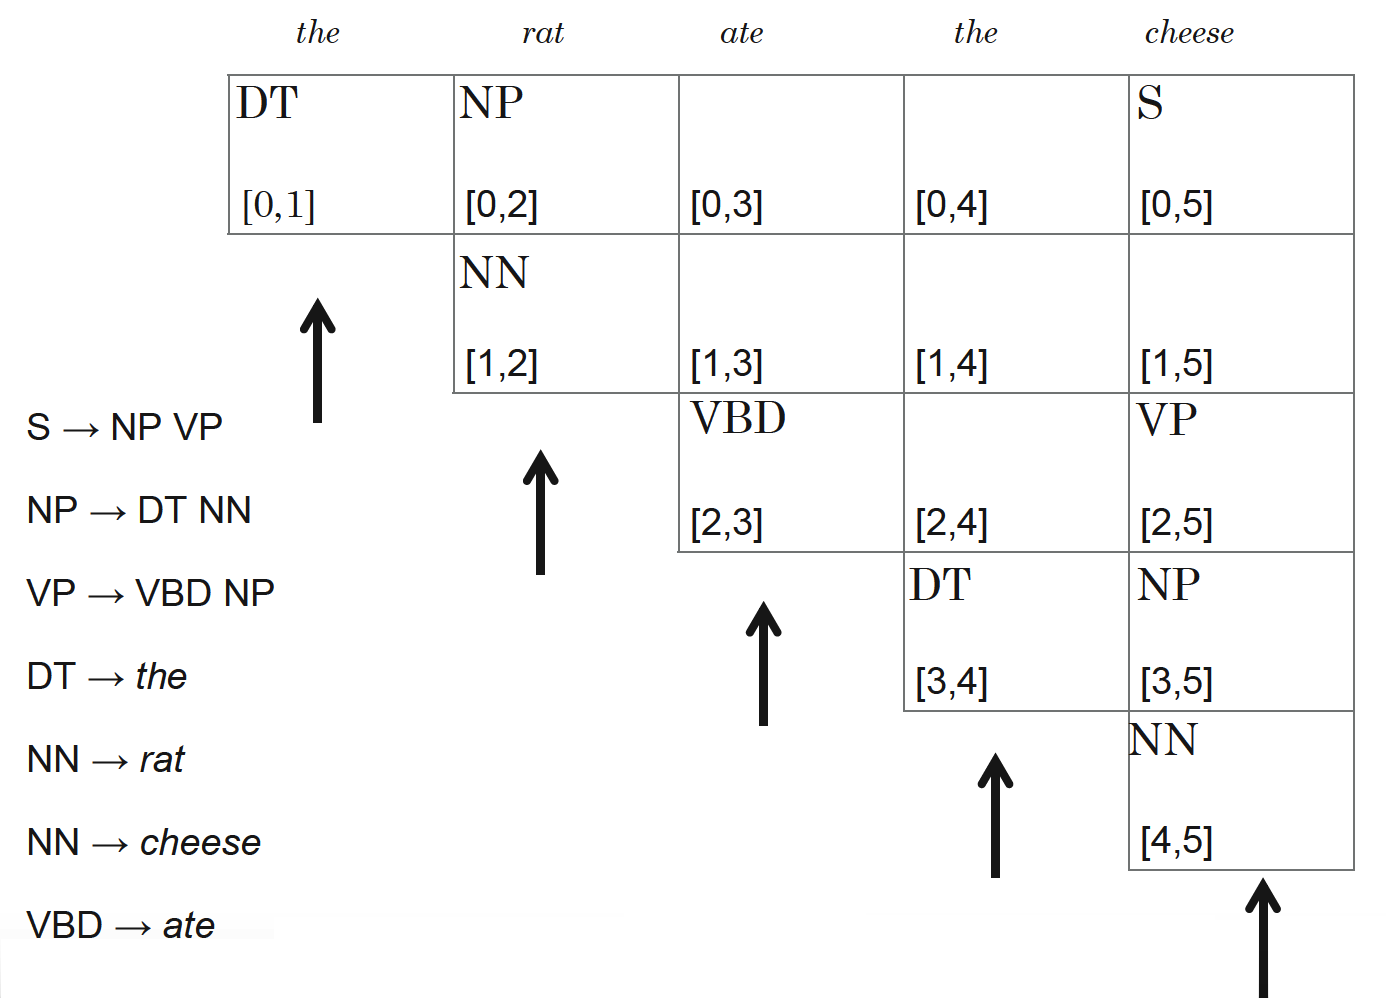
\includegraphics[width=0.8\textwidth]{include_picture/table.png} %插入图片，[]中设置图片大小，{}中是图片文件名
    \caption{CYK算法执行示例} %最终文档中希望显示的图片标题
    \label{table} %用于文内引用的标签
\end{figure}

对于这份伪代码，不难看出，其对于table的求解顺序是从左向右，自下而上的。也就是说对于这个上三角的table，算法首先求解最左侧的列，在一列求解完毕后求解右侧的列。在每一列内，算法首先求解下面的项，然后逐个向上求解。

\subsubsection{数据依赖}

由于我们要设计并行算法，因此必须考虑数据依赖问题。对于上述伪代码给出的CYK算法方案，一个table项目的求解依赖于其左侧的项目和下方的项目。在求解某个项目时，必须保证其左侧和下方的项目已经全部求解完毕。

\subsection{算法实现}

提供的文件serial\_CYK.cpp中提供了一个CYK算法的串行实现，这里对其进行梳理与解读。

\subsubsection{主要执行流程}

在完成输入后，程序首先对production1数组进行排序，并建立索引vtIndex，同时初始化表格subTreeTable，填写其对角线上的元素，即完成对单个终结符的分析。然后对production2数组排序，并建立索引vnIndex。

然后进入算法的核心部分，也就是子树生成的阶段。在该阶段中，对于表格subTreeTable中的每一个项目，也就是每一个子串的子树信息，程序首先将其存储到一个缓冲区中。在每个项目求解完毕后，将其排序，再保存到表格中。关于各个项目的求解顺序，程序实现与上述伪代码不同。在程序中，最外层循环遍历子串长度len，从2到string\_length。第二层循环遍历子串的左起始点left，从0到string\_length-len，可以通过左起始点和长度唯一的标识子串，也就是说已经定位到了表格中待求解的项目。第三层循环遍历所有可能的子串划分点right，或者说是右子串的起始点，从left+1到left+len，对于刚刚唯一确定的子串，我们需要将其划分为两部分，寻找是否有二元产生式与之对应。至此我们已经确定了子串的划分形式，第四层循环遍历左子串在表格中保存的信息，也就是遍历左子串对应的子树，而第五层循环也就是最内层循环，则遍历右子串对应的子树，最后查询产生式，寻找其是否能够规约成为一个非终结符。

最后，程序根据表格信息subTreeTable[0][string\_length-1]进行输出

\subsubsection{输入}

下发的作业说明文档中也提供了对于输入的说明。

从“input.txt”读入。第一行是一个整型，表示非终结符的数量vn\_num；第二行是一个整型，表示“右侧是两个非终结符的产生式”的数量production2\_num，即代码中的Production2类型的数量；接下来production2\_num行，每行是一个Production2类型，非终结符的格式是“<\%d>”，数字范围是0到(production2\_num-1)，“<0>”表示开始符号；然后下一行是一个整型，表示“右侧是一个终结符的产生式”的数量production1\_num，即代码中的Production1类型的数量；接下来production1\_num行，每行是一个Production1类型，终结符的格式是“\%c”，范围是所有可打印的ASCII字符；然后下一行是一个整型，表示被测试的字符串的长度；最后一行是被测试的字符串。

结合代码不难发现，我们允许产生式是无序的，一个非终结符可以生成多种串，同一种串也能够出现在不同产生式的右侧。但是终结符必须是单个可见字符。

\section{并行程序设计与实现}

\subsection{并行程序设计}

在前面的章节中，我们讨论到，提供的串行的代码在求解表格中项目时，是逐斜线求解的。在初始化的时候求解上三角阵左下方（从左上[0, 0]至右下）的对角线，然后向右上方移动。这种求解顺序非常适合并行程序，因为对于每一轮，也就是每次的一条斜线，也就是最外层循环的每一次执行，其中所有待求解项目依赖的数据都已经准备好了。而伪代码的求解顺序则不允许在同一个层次上进行并行化，因为伪代码中的求解顺序是从左至右，从下至上的。每个最外层循环的执行包含一列的项目，而上方的项目依赖下方的项目，不能在这个层次上并行。但是仍可以考虑在每个项目的求解之中并行，但这可能需要处理数据冲突。

因此，对于提供的串行代码，我就计划按上面提到的方案，串行化的执行最外层的循环，按顺序依次求解不同长度子串能够归约到的非终结符；对于每个给定的子串长度，并行化的求解不同起始位置的子串。结合表格形象的说明的话，就是并行求解一条斜线上的各个项目，然后在这一条斜线上所有的项目求解完毕后，再并行的求解下一条斜线。

\subsection{并行程序实现}

实现上述并行化设计的核心就是并行执行第二层循环，可以采用如下方案。

\begin{lstlisting}[language=C++,title={并行代码实现方案}]
    // 最外层循环，遍历子串长度
    for (int len = 2; len <= string_length; len++)
    {
        // 第二层循环，遍历子串起点
        # pragma omp parallel for num_threads(thread_count)
        for (int left = 0; left <= string_length - len; left++)
        {
\end{lstlisting}

在上述代码局部中，我在第二层循环外使用了编译器指令pragma omp parallel for，创建多个线程并行的执行第二层循环。但在课上我们提到，这样可能会导致频繁的线程create和join，带来额外的开销，因此，我使用以下这种实现方案。

\begin{lstlisting}[language=C++,title={优化后的并行代码实现方案}]
    // 最外层循环，遍历子串长度
    # pragma omp parallel num_threads(thread_count)
    for (int len = 2; len <= string_length; len++)
    {
        // 第二层循环，遍历子串起点
        # pragma omp for
        for (int left = 0; left <= string_length - len; left++)
        {
\end{lstlisting}

在这段代码中，我在进入最外层循环前，就创建了并行区域，完成了多个线程的创建，避免了在循环中频繁的创建和销毁线程。

\section{实验}

在完成了代码的并行化后，通过实验来观察并行化对程序运行时间带来的变化。

\subsection{实验环境}

程序在我个人的家用服务器上运行，处理器为英特尔® 酷睿™ i7-12700，最大睿频频率4.90 GHz，8个性能核和4个能效核，共20个线程，双通道内存共64G，DDR4 3200MHz。操作系统为Ubuntu 23.10 Server，直接运行在物理机上。程序直接运行在宿主机操作系统上，而非运行在容器中。

在进行实验时，宿主机上所有的容器均已停止，但仍有大量进程运行，只不过它们几乎不使用CPU。

\subsection{实验组别}

\subsubsection{串行执行}

串行代码处理输入文件“input2.txt”的执行时间，作为对比的基准。之后的组中都使用该文件作为输入。

\subsubsection{并行区域位于外层循环内}

使用在“并行代码实现方案”中展示的实现方式，在外层循环内创建和销毁线程。

\subsubsection{默认调度策略}

从该组开始，包括动态调度策略、默认引导式调度的各组，均使用“优化后的并行代码实现方案”中展示的实现方式，在外层循环外创建并行区域，在并行区域内再并行化第二层for循环。

这里使用默认的调度策略，即静态调度，同时不指定chunk\_size块大小。此时OpenMP会将for循环按其下标均匀的分配给各个线程执行。

\subsubsection{动态调度策略}

循环迭代被分成大小相等的块，并动态分配给线程。当一个线程完成一个块时，它会获取下一个块。在该组中，使用了默认（1），4，16三种不同的块大小进行测试。

\begin{lstlisting}[language=C++,title={块大小为4的动态调度策略}]
    // 最外层循环，遍历子串长度
    # pragma omp parallel num_threads(thread_count)
    for (int len = 2; len <= string_length; len++)
    {
        // 第二层循环，遍历子串起点
        # pragma omp for schedule(dynamic, 4)
        for (int left = 0; left <= string_length - len; left++)
        {
\end{lstlisting}

\subsubsection{默认引导式调度}

类似于dynamic，但块的大小逐渐减小。初始块较大，后续块逐渐变小，直到达到指定的chunk\_size。这里没有指定块大小，默认为1。

\begin{lstlisting}[language=C++,title={默认引导式调度}]
    // 最外层循环，遍历子串长度
    # pragma omp parallel num_threads(thread_count)
    for (int len = 2; len <= string_length; len++)
    {
        // 第二层循环，遍历子串起点
        # pragma omp for schedule(guided)
        for (int left = 0; left <= string_length - len; left++)
        {
\end{lstlisting}

\subsection{实验数据记录表}

单位为微秒。

\begin{table}[H]
\tiny
\caption{实验数据记录表}
\centering
\begin{tabular}{lrrrrrr}
\hline  
\textbf{组别} & \textbf{数据1} & \textbf{数据2} & \textbf{数据3} & \textbf{数据4} & \textbf{数据5} & \textbf{平均}\\ 
\hline  
串行程序 & 47290223 & 47429547 & 47243947 & 47294040 & 46829509 & 47217453.2 \\
并行区域位于外层循环内（线程数1） & 50109798 & 50566555 & 49595740 & 49606736 & 49577341 & 49891234 \\
并行区域位于外层循环内（线程数2） & 25560577 & 25904316 & 25632841 & 25627501 & 25563017 & 25657650.4 \\
并行区域位于外层循环内（线程数4） & 13189456 & 13153158 & 13225255 & 13200646 & 13222267 & 13198156.4 \\
并行区域位于外层循环内（线程数8） & 7052946 & 7013102 & 6991525 & 6971041 & 6980119 & 7001746.6 \\
并行区域位于外层循环内（线程数16） & 6486875 & 6449169 & 6482928 & 6435375 & 6428611 & 6456591.6 \\
并行区域位于外层循环内（线程数32） & 6276551 & 6163628 & 6202596 & 6217395 & 6172942 & 6206622.4 \\
默认调度策略（线程数1） & 50216643 & 49604925 & 49733300 & 49642874 & 51016855 & 50042919.4 \\
默认调度策略（线程数2） & 26177365 & 25596754 & 25536314 & 26180371 & 25952469 & 25888654.6 \\
默认调度策略（线程数4） & 13165393 & 13158068 & 13243478 & 13167513 & 13173469 & 13181584.2 \\
默认调度策略（线程数8） & 6953577 & 6950707 & 6938714 & 7037207 & 6992164 & 6974473.8 \\
默认调度策略（线程数16） & 6492385 & 6503187 & 6465681 & 6573176 & 6604548 & 6527795.4 \\
默认调度策略（线程数32） & 5660697 & 5573832 & 5564571 & 5533691 & 5582940 & 5583146.2 \\
默认动态调度策略（线程数1） & 48919220 & 48900132 & 48842425 & 48850797 & 49992504 & 49101015.6 \\
默认动态调度策略（线程数2） & 25090084 & 25113430 & 25393433 & 25083938 & 25355806 & 25207338.2 \\
默认动态调度策略（线程数4） & 13005568 & 12914429 & 12963346 & 12949802 & 13041973 & 12975023.6 \\
默认动态调度策略（线程数8） & 6842167 & 6817261 & 6844541 & 6839818 & 6843544 & 6837466.2 \\
默认动态调度策略（线程数16） & 5053150 & 5010014 & 5025454 & 5047820 & 5157809 & 5058849.4 \\
默认动态调度策略（线程数32） & 4857386 & 4862722 & 4850516 & 4938866 & 4979993 & 4897896.6 \\
块大小为4的动态调度策略（线程数1） & 48874635 & 49364019 & 50162451 & 48816863 & 49039505 & 49251494.6 \\
块大小为4的动态调度策略（线程数2） & 25338184 & 25547935 & 25259233 & 25287723 & 25275920 & 25341799 \\
块大小为4的动态调度策略（线程数4） & 13147614 & 13201528 & 13143122 & 13191606 & 13179603 & 13172694.6 \\
块大小为4的动态调度策略（线程数8） & 7125111 & 7109418 & 7110982 & 7117465 & 7107781 & 7114151.4 \\
块大小为4的动态调度策略（线程数16） & 5559692 & 5608104 & 5565223 & 5554065 & 5563028 & 5570022.4 \\
块大小为4的动态调度策略（线程数32） & 5422694 & 5428728 & 5392114 & 5423129 & 5416209 & 5416574.8 \\
块大小为16的动态调度策略（线程数1） & 50174676 & 49163463 & 49024093 & 48977602 & 49081626 & 49284292 \\
块大小为16的动态调度策略（线程数2） & 25758806 & 25876862 & 25795849 & 25953303 & 25897297 & 25856423.4 \\
块大小为16的动态调度策略（线程数4） & 14046048 & 13987214 & 14062960 & 14085373 & 14095462 & 14055411.4 \\
块大小为16的动态调度策略（线程数8） & 8243259 & 8249818 & 8245257 & 8234858 & 8250609 & 8244760.2 \\
块大小为16的动态调度策略（线程数16） & 7620321 & 7590981 & 7636432 & 7656990 & 7578567 & 7616658.2 \\
块大小为16的动态调度策略（线程数32） & 7209361 & 7128360 & 7075783 & 7158845 & 7061271 & 7126724 \\
默认引导式调度（线程数1） & 49023811 & 50161119 & 49547991 & 48971514 & 48859851 & 49312857.2 \\
默认引导式调度（线程数2） & 25124326 & 25300796 & 25117492 & 25116556 & 25275798 & 25186993.6 \\
默认引导式调度（线程数4） & 12911455 & 12928859 & 13018339 & 12901014 & 12905975 & 12933128.4 \\
默认引导式调度（线程数8） & 6831869 & 6839402 & 6809426 & 6824238 & 6812803 & 6823547.6 \\
默认引导式调度（线程数16） & 5738434 & 5683263 & 5690302 & 5838473 & 5854713 & 5761037 \\
默认引导式调度（线程数32） & 5344789 & 5286660 & 5264765 & 5366594 & 5775076 & 5407576.8 \\

\hline
\end{tabular} 
\end{table}

\section{问题的回答}

\subsection{如何将任务进行分块的？}

这个问题在“并行程序设计”一节中进行了详细解释。

\subsection{如何提升运行速度与增强程序扩展性？}

串行化本身就可以提升运行速度，可以通过调整数据的划分，并行化的实现方案，线程间的调度算法等等来进一步优化。此外，也可以使用更强大的处理器，进一步优化算法等来提高运行速度，如代码中已经实现的产生式排序和索引。

目前的程序仅仅支持上下文无关文法，但这是CYK算法本身决定的，暂且不讨论。在“算法实现”一节中也讨论了程序输入的约束，目前终结符仅仅支持单个字符，可以对其进行略微修改，使用长整型等表示终结符。这样我们既可以将其映射到字符，直接表示终结符，也可以令其表示词素，使得程序可以与词法分析器对接，支持更加复杂的文法。

\subsection{如何测量程序运行时间？}

我使用chrono，在程序内部添加代码，以输出主要部分的执行时间。

\begin{lstlisting}[language=C++,title={时间记录代码}]
#include <iostream>
#include <chrono>

using namespace std;
using namespace std::chrono;

int main() {
    /* 读取输入文件 */

    // 记录开始时间
    auto start = high_resolution_clock::now();

    /* 建立产生式索引 */
    /* 执行CYK算法 */
    
    auto stop = high_resolution_clock::now();
    auto duration = duration_cast<microseconds>(stop - start);

    /* 输出CYK算法结果 */

    // 输出运行时间
    cout << "time: " << duration.count() << " us" << endl;

    return 0;
}
\end{lstlisting}

\subsection{比较图}

以下是不同组别方案的耗时时间比较图，单位是微秒。具体各个组内的实现方案在“实验组别”一节中进行了介绍。

\begin{figure}[H] %H为当前位置，!htb为忽略美学标准，htbp为浮动图形
    \centering %图片居中
    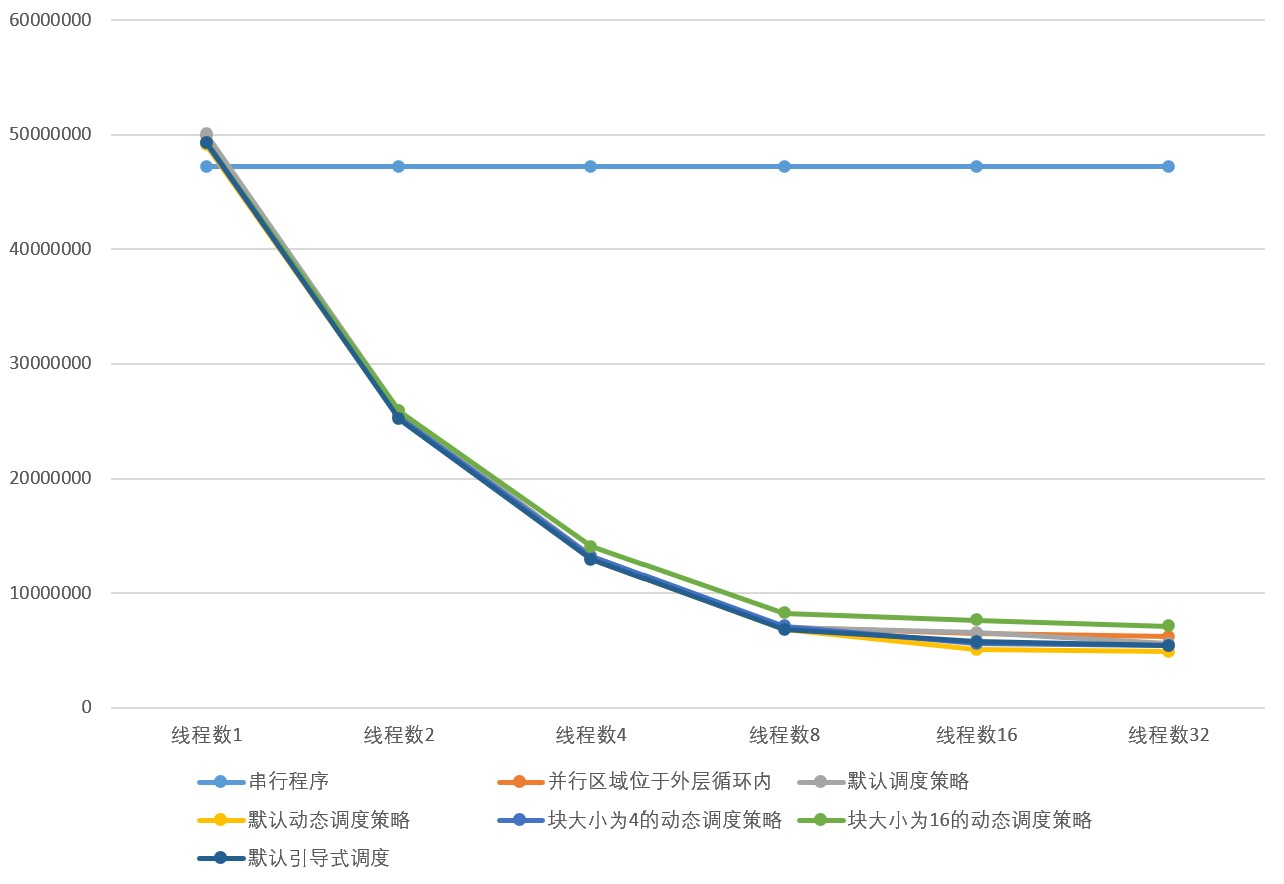
\includegraphics[width=0.8\textwidth]{include_picture/time.jpg} %插入图片，[]中设置图片大小，{}中是图片文件名
    \caption{耗时比较折线图} %最终文档中希望显示的图片标题
    \label{time} %用于文内引用的标签
\end{figure}

\begin{figure}[H] %H为当前位置，!htb为忽略美学标准，htbp为浮动图形
    \centering %图片居中
    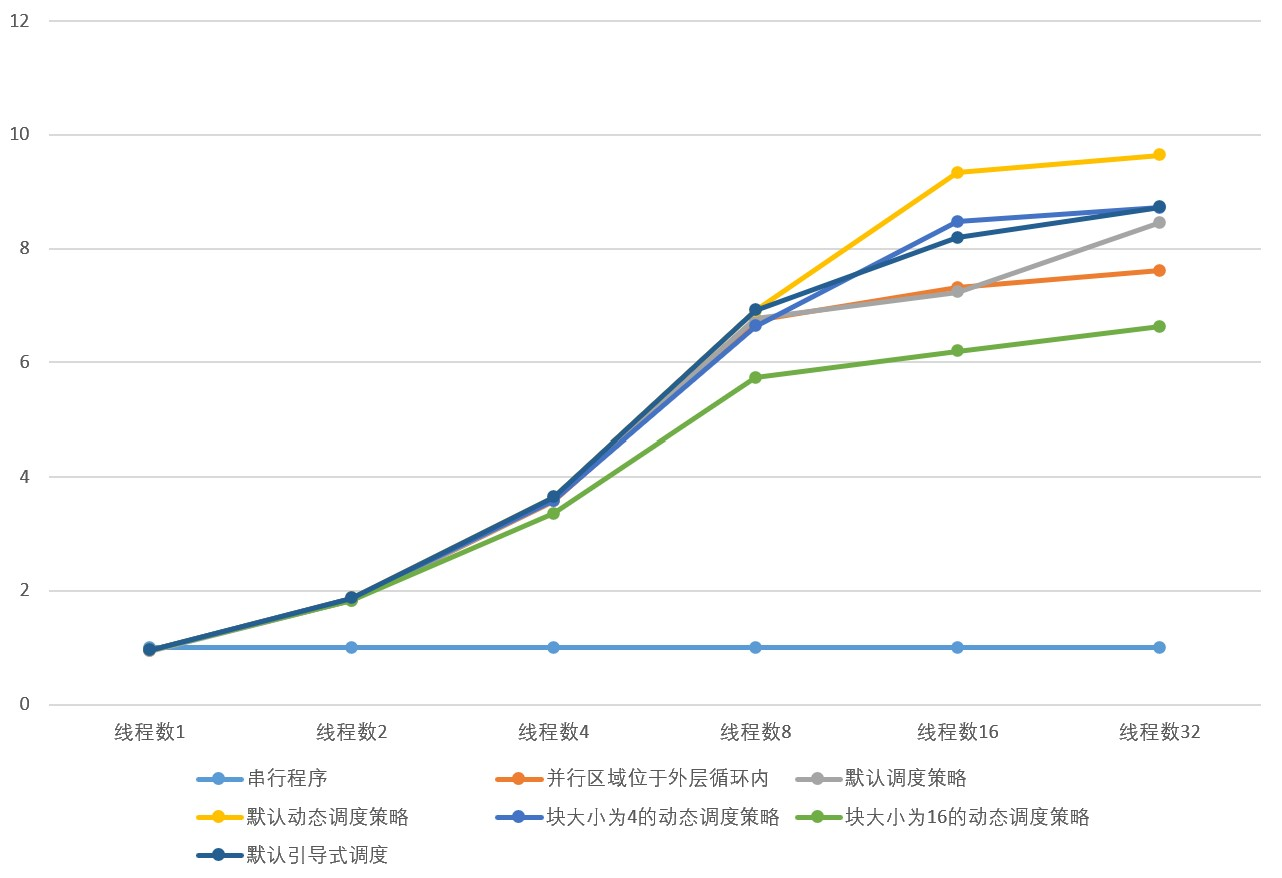
\includegraphics[width=0.8\textwidth]{include_picture/rate.jpg} %插入图片，[]中设置图片大小，{}中是图片文件名
    \caption{加速比比较折线图} %最终文档中希望显示的图片标题
    \label{rate} %用于文内引用的标签
\end{figure}

\subsection{加速比变化的趋势}

通过观察图\ref{time}和图\ref{rate}，可以发现随着线程数的增加，并行策略的加速比呈现上升趋势，说明并行化在一定程度上提高了程序的执行效率。在低线程数（如线程数2和线程数4）时，加速比增长较快，体现了并行化的初步优势。在较高线程数（如线程数16和线程数32）时，加速比的增长开始放缓，甚至出现下降的趋势，这可能是由于并行化带来的开销（如线程管理、同步等）超过了计算的加速收益，以及仅有20个物理线程的限制。

通过对比“并行区域位于外层循环内”和“默认调度策略”两条线，可以发现似乎将线程的创建和销毁移动到最外层循环外并没有明显的作用，这可能是由于最外层的循环并不会执行非常多次，且线程的创建和销毁相比于任务本身，花费很小导致的。

默认的动态调度策略表现比默认调度策略好，可以说明任务的花费不太均匀，动态分配任务的收益大于调度的额外开销。随着块大小的增大，动态分配策略表现的越来越差，这很可能是较大的任务块使得对于各个线程任务分配的不均匀，尤其是当算法执行到后面时，每个循环中需要并行的任务数量（下标）并不多，较大的块大小甚至可能导致有大量线程闲置。

引导式调度策略表现一般，进一步印证对于该任务，调度的花费其实并不高，小于任务分配不均带来的额外开销，不需要开始使用大块来减轻调度任务，更精细的调度策略可能是更好的选择。

\subsection{最佳方案}

最佳的方案是使用默认的动态调度策略，已经在上一节中进行了分析。

\end{spacing}



\end{document}
